\chapter{Installationsanleitung}
Da verschiedene Technologien zum Umsetzten des Projektes beziehungsweise der Anwendungen genutzt wurden folgt nun für jedes eingesetzte Werkzeug eine kompakte Installationsanleitung. Eine Installationsanleitung ist notwendig, da je nach Werkzeug einige Besonderheiten bei der Installation zu beachtet sind. Außerdem werden je nach Werkzeug zusätzliche Plugins oder Erweiterungen benötigt, um die Anwendung auf einem andern Host-System erfolgreich ausführen zu können.
\\\\
Wichtig an dieser Stelle ist, dass diese Installationsanleitung nur für Nutzer mit dem Betriebssystem "Windows 10 Pro"{} verfasst wurde. Da auf allen verwendeten Host-Systemen dieses Betriebssystem installiert war. Nach aktuellen Erkenntnissen sollte es jedoch kein Problem sein die in diesem Projekt genutzten Programme und Tools auch auf einem anderen Betriebssystem zu installieren. In diesem Fall verweisen wir jedoch auf die von den Herstellern bereitgestellten Installationsanleitungen.
\\\\
Zunächst werden wir alle benötigten Programme und Abhängigkeiten installieren und anschließen wird erklärt wie der Server und die Ionic-Anwendung gestartet werden kann.
\\\\
Neben den hier vorgestellten Tools und Werkzeugen wurde Visual Studio Code (VS Code) als Entwicklungsumgebung für das Projekt genutzt. VS Code hat den Vorteil ein schlankes und leichtgewichtige Anwendungen zu sein, welche mittels Plugins (Extension) um benötigte Funktionen erweiterbar ist. Es kann sowohl zum Entwickeln und Starten des Backends als auch für das Frontend genutzt werden.

\subsection{Projektstruktur}\label{Projektstruktur}
Das Projekt besteht aus drei Hauptordnern: Backend, Frontend und Dokumentation. In dem Ordner Backend befinden sich alle für den Server benötigte Daten. Im Ordner Frontend alle Daten für die Ionic-Anwendung und im Ordner Dokumentation alle Materialien zur Dokumentation.
\section{Docker}\label{DockerInstal}

Docker vereinfacht die Anwendungsbereitstellung, indem es den Transport und die Installation von Containern erleichtert, die alle erforderlichen Pakete als Dateien enthalten. Container gewährleisten die Trennung und Verwaltung der auf einem Computer verwendeten Ressourcen. Dazu gehören nach Angaben der Entwickler: Code, Laufzeitmodul, Systemwerkzeuge, Systembibliotheken - eben alles, was auf einem Computer installiert werden kann.
\begin{enumerate}
    \item Zunächst muss der Installations-Client für \href{https://docs.docker.com/docker-for-windows/install/}{Docker} heruntergeladen werden. Den Link dazu finden Sie hier:\href{https://docs.docker.com/docker-for-windows/install/}{https://docs.docker.com/docker-for-windows/install/}\\\\\textcolor{red}{Wichtig:} Für Windows wird entweder die Pro, Enterprise oder Education Version benötigt.
    
    \item Während der Installation von Docker werden Sie gefragt, ob Sie Windows Container oder Linux Container verwenden möchten. Stellen Sie sicher, dass Sie das Kästchen in der angezeigten Option nicht ankreuzen (vgl. Abbildung). Der Docker verwendet also Linux Contrainer. Docker-Container verwenden oft Linux-Komponenten, womit Windows-Container oft Probleme haben.\\
    \begin{center}
        \begin{minipage}[t]{0.5\textwidth}
            \centering
            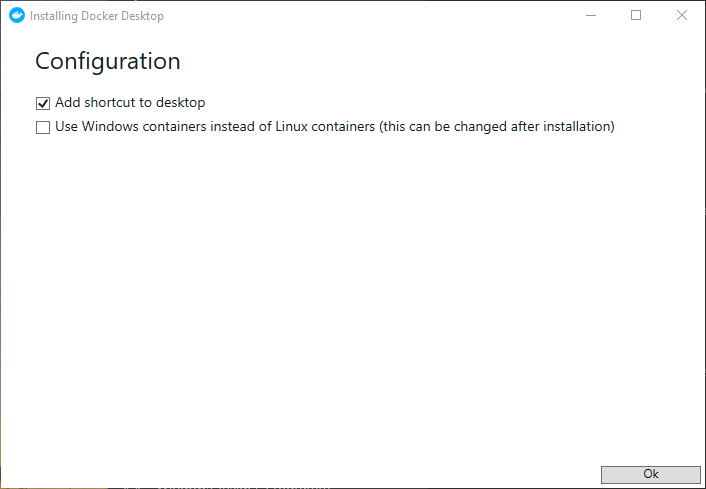
\includegraphics[width=(\textwidth)]{Kapitel3/DockerConfig.png}
            \captionof{figure}{Das Feld "Windows-Containers" sollte frei bleiben.}
            \label{ContainerConfig}
        \end{minipage}
    \end{center}

    \item Unter Windows müssen Sie Hyper-V und Container aktivieren. Hyper-V und Container können unter den Windows-Funktionen aktiviert werden. Dazu drücken Sie zunächst die Windows-Taste + Q und geben dort die Windows-Features ein. Aktivieren Sie dann Hyper-V und Container und klicken Sie auf "OK". Folgen Sie dann der Windows-Installation und installieren Sie die Features. Nach der Installation der Windows-Features müssen Sie den PC neu starten.\\\\\textcolor{red}{Wichtig:} Um Virtualisierungsdienste nutzten zu können, müssen diese gegebenenfalls im Bios-System aktiviert werden.
    \begin{center}
        \begin{minipage}[t]{0.35\textwidth}
            \centering
            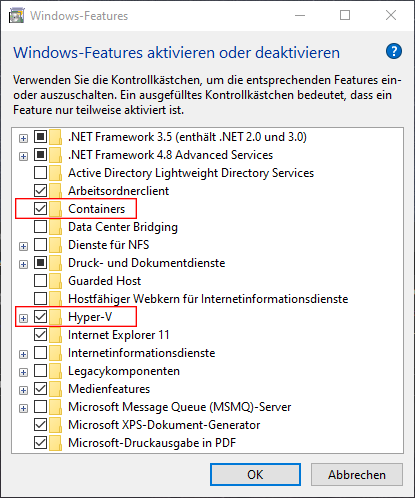
\includegraphics[width=(\textwidth)]{Kapitel3/WinFeature.png}
            \captionof{figure}{Benötigte Windows Features - Containers und Hyper-V.}
            \label{ContainerConfig}
        \end{minipage}
    \end{center}

    \item Es biete sich an unter Windows die "Windows PowerShell"{} zu nutzen, da diese für Docker nützliche Funktionalitäten im Gegensatz zur einfachen "Eingabeaufforderung"{} mit bringt. Wenn die Windows PowerShell noch nicht installiert wurde, können Sie es mit den Windows-Funktionen installieren. Drücken Sie dazu zunächst die Windows-Taste + Q und geben Sie "Windows-Feature" ein. Schalten Sie dann Windows PowerShell ein, und drücken Sie dann "OK". Installieren Sie PowerShell und starten Sie dann den Computer neu. 

    \begin{center}
        \begin{minipage}[t]{0.4\textwidth}
            \centering
            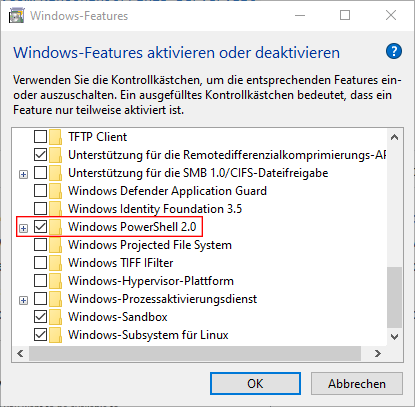
\includegraphics[width=(\textwidth)]{Kapitel3/WinPowerShell.png}
            \captionof{figure}{Benötigte Windows Features - PowerShell.}
            \label{ContainerConfig}
        \end{minipage}
    \end{center}


    \item Um nun einen Docker-Container unter Windows nutzen zu können, benötigt Docker noch Zugriff auf den Speicherort, auf welchem sich der Docker-Container befindet. Hierzu muss Docker Zugriff auf die Festplattenpartition gewährt werden, auf der die Docker-Container gespeichert sind. Um dies zu ermöglichen muss mit der linken Maustaste auf das Docker-Symbol in der Taskleiste das Einstellungsmenü geöffnet werden. Anschließen navigieren Sie zu dem Reiter "Resources / File Sharing"{}. Dort können Sie Docker Zugriff auf die Partitionen gewähren oder Sie wieder aufrufen. An diesem Punkt werden Sie auch nach dem aktuellen Windows-Benutzerkennwort gefragt. Sollten sie nach einem Passwort gefragt werden, geben Sie Ihr aktuelles Windows-Passwort ein, um Docker Zugriff auf die Partition zu gewähren. 
    
    \begin{center}
        \begin{minipage}[t]{0.8\textwidth}
            \centering
            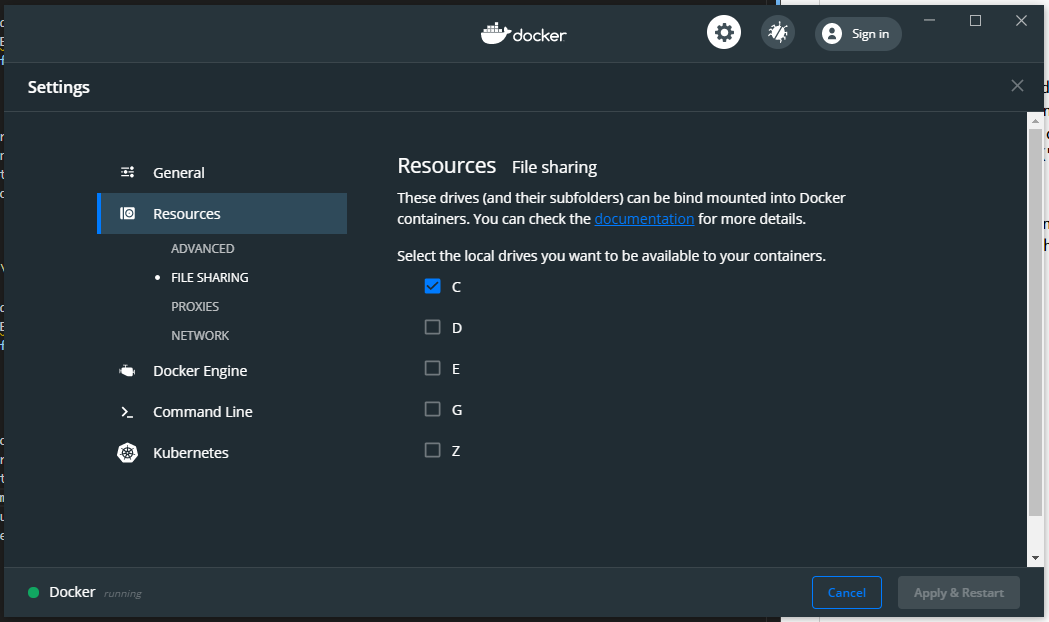
\includegraphics[width=(\textwidth)]{Kapitel3/DockerFiles.png}
            \captionof{figure}{Freigabe einzelner Partitionen für Docker.}
            \label{ContainerConfig}
        \end{minipage}
    \end{center}

\end{enumerate}

\section{Spring Boot}\label{SpringInstal}

Wurde Docker erfolgreich installiert erfolgt nun die Anleitung zur Installation und Inbetriebnahme der Spring Boot Anwendung.
Die Installation zu Spring Boot ist recht einfach dazu benötigen wir lediglich das Java Developer Kit 1.8 und  Build-Management-Tool Maven.

\begin{enumerate}
    \item Die Installationsanwendung zu Java Developer Kit 1.8 kann unter folgendem Link aufgerufen werden:\\\href{https://www.oracle.com/java/technologies/javase-jdk8-downloads.html}{https://www.oracle.com/java/technologies/javase-jdk8-downloads.html}
    
    \item Im nächsten Schritt wird zunächst Maven heruntergeladen. Mit Maven kann man insbesondere Java-Programme standardisiert erstellen und verwalten. Den Link dazu finden Sie hier: \href{https://mirror.dkd.de/apache/maven/maven-3/3.6.3/binaries/apache-maven-3.6.3-bin.zip}{https://mirror.dkd.de/apache/maven/maven-3/3.6.3/binaries/apache-maven-3.6.3-bin.zip}.\\\\\textcolor{red}{Wichtig:} Es sollte darauf geachtet werden, dass die Binaries heruntergeladen werden. Diese enthalten einen Ordner mit der Bezeichnung "bin"{}, welcher für spätere Zwecke benötigt wird.
    
    \item Nachdem die Binaries heruntergeladen wurden, entpacken wir den Ordner. Da Maven jedes Mal wenn das Programm kompiliert werden soll benötigt wird, bietet es sich an den Ordner dauerhaft an einen "sicheren"{} Ort abzuspeichern. Es bietet sich an Maven in den Umgebungsvariable bekannt zu machen. Dadurch muss nicht bei jedem Maven-Befehl der korrekte Pfad zu den entpackten Ordner angegeben werden. Ist Maven dem System bekannt, wird wenn ein Maven-Befehl aufgerufen wird, der Pfad zum entpackten Ordner automatisch durch das System hinzugefügt.
    
    \item Nun öffnen Sie per Windows-Taste + Q das Suchfeld und suchen dort nach "{}Systemumgebungsvariablen bearbeiten"{} . Es sollte sich nun ein Fenster öffnen. Dort drücken Sie auf "Umgebungsvariablen bearbeiten"{}.
    
    \begin{center}
        \begin{minipage}[t]{0.5\textwidth}
            \centering
            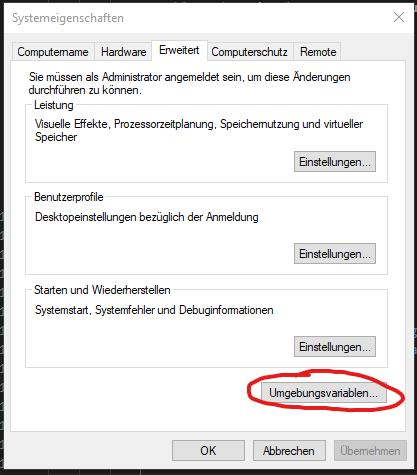
\includegraphics[width=(\textwidth)]{Kapitel3/SpringUmgebung.png}
            \captionof{figure}{Umgebungsvariable bearbeiten.}
            \label{ContainerConfig}
        \end{minipage}
    \end{center}

    \item Im nächsten Fenster wählen Sie zunächst unter Systemvariablen den Wert Path aus und drücken dann auf bearbeiten.
    
    \begin{center}
        \begin{minipage}[t]{0.5\textwidth}
            \centering
            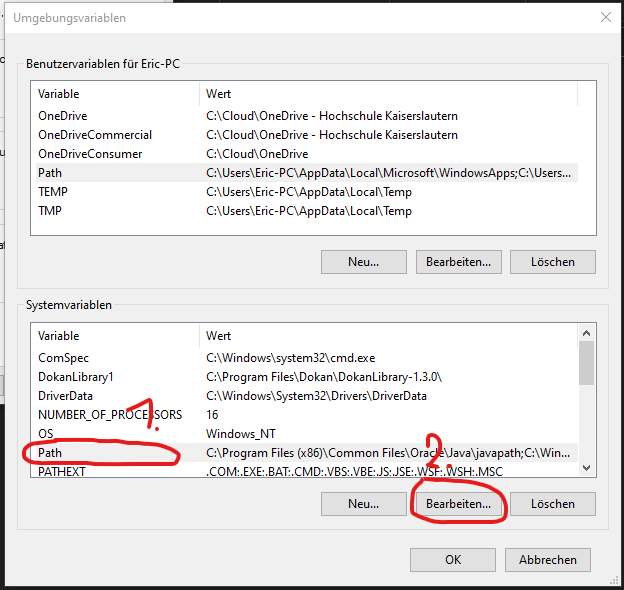
\includegraphics[width=(\textwidth)]{Kapitel3/SpringBearbeiten.png}
            \captionof{figure}{Umgebungsvariable bearbeiten.}
            \label{ContainerConfig}
        \end{minipage}
    \end{center}

    
    \item Dort fügen Sie mit "Neu"{} einen neuen Eintrag in der Tabelle hinzu und können nach auswählen der neuen Spalte über "Durchsuchen"{} den Pfad zu dem Maven-Ordner angeben.\\\\\textcolor{red}{Wichtig:} Zu beachten ist, dass der Ordner "bin"{} auf jeden Fall angegeben werden muss. Ansonsten kann Windows die benötigten Dateien nicht finden.

    \begin{center}
        \begin{minipage}[t]{0.5\textwidth}
            \centering
            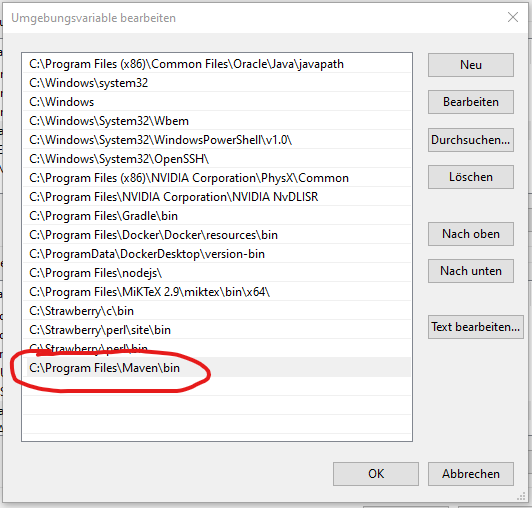
\includegraphics[width=(\textwidth)]{Kapitel3/SpringAdd.png}
            \captionof{figure}{Umgebungsvariable hinzufügen.}
            \label{ContainerConfig}
        \end{minipage}
    \end{center}
\end{enumerate}


\section{Ionic}\label{IonicInstal}

Um eine Ionic-Anwendung zu programmieren wird neben einer Entwicklungsumgebung lediglich NodeJS und einige Erweiterungen benötigt.

\begin{enumerate}
    \item Der erste Schritt ist das Herunterladen und Installieren von Node.JS. Sie finden Node.JS unter folgendem Link:
    \href{https://nodejs.org/en/download/current/}{https://nodejs.org/en/download/current/}    
    
    \item Starten Sie nach der Installation von Node.JS die Eingabeaufforderung oder Windows PowerShell und geben Sie den Befehl \underline{npm --version} ein. Wenn Sie die aktuelle Versionsnummer sehen, wurde Node.JS korrekt installiert. 

    \item  Nun müssen noch Ionic und Cordova installiert werden. Geben Sie zunächst an der Eingabeaufforderung \underline{npm install -g cordova} ein. Dadurch wird das Cordova-Framework installiert, das später für die Bereitstellung der Anwendung auf verschiedenen Plattformen benötigt wird. Danach benötigen Sie das Ionic-Framework, um Anwendungen in Ionic zu erstellen. Sie können Ionic mit dem Befehl \underline{npm install -g ionic} installieren. 
    
    \item Ionic unterstützt verschiedene Programmiersprachen. Standardmäßig werden Ionic-Anwendungen in JavaScript programmiert. Es ist jedoch auch möglich Ionic-Anwendungen in Angular, React oder Vue zu programmieren. Um Ionic-Anwendungen in anderen Sprachen programmieren zu können, müssen Sie auch die entsprechende CLI auf Ihrem System installieren. Für dieses Projekt wurde die TypScript-Sprache Angular genutzt. Um Angular zu installieren muss folgender Befehl eingegeben werden: \underline{npm install –g @angular/cli}  
    
    \item Nach der Installation von Angular starten Sie die Eingabeaufforderung oder Windows PowerShell und navigieren sich in den "Frontend" Ordner des Projektes. Führen Sie dort die folgenden Befehle aus:\\
    -- \underline{npm install}\\
    -- \underline{npm cache verify}\\
    Mit diesen Befehlen installieren sie alle benötigten Abhängigkeiten für das kompilieren und ausführen von Ionic- beziehungsweise Angular-Anwendungen.

    
\end{enumerate}{}
Im zweiten Schritt werden nun alle Plugins installieren, die Ionic zur Unterstützung von anderen Plattformen benötigt.

\begin{enumerate}
    \item Damit Ihre Ionic-Anwendung eine Plattform unterstützt, öffnen Sie zunächst die Eingabeaufforderung und wechseln Sie in das aktuelle Verzeichnis Ihres Ionic-Projekts. 
    
    \item Geben Sie folgenden Befehle ein um IOS als Ziel-Plattform hinzuzufügen: \underline{ionic cordova platform add ios}
    \item Geben Sie folgenden Befehle ein um Android als Ziel-Plattform hinzuzufügen: \underline{ionic cordova platform add android}
    \item Anschließend müssen noch die Ressourcen der Plattform hinzugefügt werden. Hierzu muss der Befehl \underline{npm install -g cordova-res} ausgeführt werden.
    
\end{enumerate}{}
Zur Unterstützung der Anwendung direkt auf einem Android-Gerät werden noch einige Programme benötigt.

\begin{enumerate}
    \item  Zunächst benötigen Sie Android Studio. Eine Einführung in die Installation und Einrichtung finden Sie unter
    \href{https://ionicframework.com/docs/developing/android}{https://ionicframework.com/docs/developing/android}
    
    \item Wurde Android Studie und alle benötigten Feature installiert, kann die Anwendung für Android Geräte gebuildet und anschließend verteilt werden. Dazu geben Sie den Befehlt \underline{ionic cordova build android} und anschließend \underline{ionic cordova emulate android} ein.\\\\
    \textcolor{green}{Alternativ} zu einem Emulator können Sie auch Ihr eigenes Android-Smartphone über USB an Ihren PC anschließen und Ihre Ionic-App auf Ihrem eigenen Telefon installieren. Siehe: \href{https://javatutorial.net/connect-android-device-android-studio}{https://javatutorial.net/connect-android-device-android-studio}

\end{enumerate}{}
Zur Unterstützung der IOS-Plattform benötigen Sie einen Computer mit MAC-OS und installiertem XCode. Eine Einführung in die Installation und Einrichtung finden Sie unter: \href{https://ionicframework.com/docs/developing/ios}{https://ionicframework.com/docs/developing/ios}

\subsection{Fehlerbehandlung}\label{IonicFehler}
Ein häufiger Fehler der beim Verteilen beziehungsweise neu Einrichten von Ionic-Projekten passiert ist das Abhängigkeiten nicht korrekt aufgelöst werden können. Oft genügt es lediglich im Ordner "Frontend" die Datei \underline{package-lock.json} und den Ordner \underline{node\_modules} zu löschen und anschließend neu zu laden. Hierzu müssen folgende zwei Befehle über die Eingabeaufforderung oder PowerShell (im Projektordner) ausgeführt werden:\\
-- npm install\\
-- npm cache verify
\\\\
Ein weitere Fehler der auftreten kann ist, dass beim Builden von Android das Programm mit dem Fehler "Gradle could not be found." fehlschlägt. In diesem Fall müssen Sie Gradle Herunterladen laden, entpacken und wie in Kapitel \ref{SpringInstal} (ab Punkt 4) dem Build-Management-Tool Maven dem System über die Umgebungsvariablen bekannt machen. 
\section{Ausführen}\label{ProjektStart}
Im folgenden Abschnitt wird kurz erklärt, wie man zunächst den Server startet und anschließen die Ionic-Anwendung über einen Browser darstellen kann. Sollte VS Code als Entwicklungsumgebung genutzt werden, bietet es sich an eine Instanz von VS Code für das Backend und eine Instanz von VS Code für das Frontend zu starten.

\subsection{Start Backend}
\begin{enumerate}
    \item VS Code bietet im Reiter den Punkt "Terminal"{} an. Darüber kann direkt in VS Code ein Terminal geöffnet werden. Das Terminal befindet sich schon im richtigen Ordner. Alternativ kann auch die Eingabeaufforderung oder die PowerShell gestartet werden und in den Projektordner "Backend" navigiert werden.
    
    \item Im ersten Schritt wechseln Sie in den Ordner vorhanden "rest\_controller"{}.\\Befehl: "cd rest\_controller"{}
    
    \item Zunächst muss das Projekt kompiliert werden. Dies kann per Befehl "mvn clean | mvn package"{} ausgeführt werden.\\\textcolor{red}{Wichtig:} Maven muss auf dem System vorhanden und über die Umgebungsvariablen dem System bekannt sein.
    
    \item Wurde das Projekt erfolgreich kompiliert, kann der Server per folgendem Befehl gestartet werden: "docker-compose up --build"{}\\
    Auch hier sei zu beachten, das sich zum einen das Terminal im Ordner "rest\_controller"{} befinden sollte und zum anderen der Docker-Deamon (Docker.exe) gestartet ist. Das Starten des Servers kann je nach Hardware einige Minuten benötigen.
\end{enumerate}


\subsection{Start Frontend}

\begin{enumerate}
    \item Auch beim Starten des Frontends wird zunächst ein neues Terminal geöffnet. Wahlweise durch VS Code oder durch Starten eines eigenen Terminal Clients. 
    
    \item Zum starten der Ionic-Anwendung muss jedoch nur der Befehlt "{}ionic serve --lab"{} ausgeführt werden. Ionic übernimmt alle weiteren Schritte zum Starten der Ionic-Anwendung. Diese wird auch automatisch im Webbrowser geöffnet, sobald alle Daten kompiliert wurden. Wird der Befehlt "{}ionic serve --lab"{} zum ersten Mal ausgeführt, kann es sein, dass Sie noch einige Abhängigkeiten installieren müssen.
    
\end{enumerate}

\subsection{Fehlerbehandlung}\label{SpringFehler}
Ein möglicher Fehler der Auftreten kann, wäre dass Spring Boot den Pfad zur JDK nicht findet und beim compilieren der Spring Boot Anwendung mit der Fehlermeldung "No compiler is provided in this environment. Perhaps you are running on a JRE rather than a JDK?"{} abstürzt. 
\\\\
In diesem Fall muss in der pom-Datein des Servers die Pfad-Angabe des JDK angepasst werden. Die pom-Datei befindet sich im Ordner "Backend\textbackslash{}rest\_controller\textbackslash{}"{}.

\begin{center}
    \begin{minipage}[t]{0.8\textwidth}
        \centering
        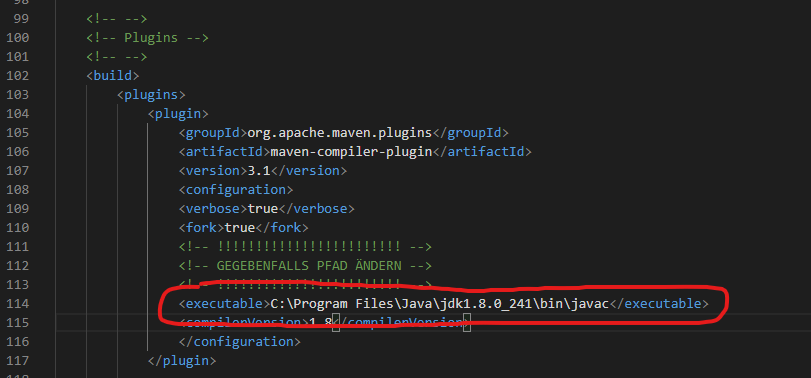
\includegraphics[width=(\textwidth)]{Kapitel3/SpringFehler.png}
        \captionof{figure}{Path-Angabe zur JDK muss angepasst werden.}
        \label{ContainerConfig}
    \end{minipage}
\end{center}
Ein weiterer Fehler könnte der sogenannte CORS-Fehler der Ionic beim Ausführen der Ionic-Anwendung im Browser auftreten kann. Die gemeinsame Nutzung von Ressourcen aus verschiedenen Quellen (Cross-Origin Resource Sharing, CORS) ist ein Standard, der es einem Server erlaubt, die Politik der gleichen Herkunft zu lockern. Dies wird verwendet, um einige Anfragen aus verschiedenen Quellen explizit zuzulassen und andere abzulehnen. Wenn eine Website beispielsweise einen integrierbaren Dienst anbietet, kann es notwendig sein, bestimmte Einschränkungen zu freizugeben. \cite{Mozilla.10.04.2020}\\\\Eine mögliche Fehler-Quelle kann sein, dass der Browser CORS-Anfrage ablehnt. Je nach Browser zum Beispiel Chrome werden einige Plugins angeboten, welche ermöglichen CORS-Anfrage zu versenden und zu empfangen. Für Google Chrome wäre dies "Allow CORS: Access-Control-Allow-Origin"{}. Aber auch für Firefox sollte ein ähnliches Plugin zur Verfügung stehen.